\chapter{第一门编程语言选谁?}

\begin{center}
第一门编程语言选谁?\cite{first_programming_language} \\ 金旭亮
\end{center}

说明:

这篇文章是专门针对大学低年级学生(和其他软件开发初学者)写的,如果你己经是研究生或本科高年级学生,请将这篇文章转发给你的师弟或师妹,希望这篇文章能够帮助他们少走弯路,顺利地迈入软件开发的大门;如果您是一位有经验的软件开发者,或者是关注计算机教育的同行,也敬请提出宝贵意见。

发表看法请在本贴评论,或者在我的新浪微博“\href{http://weibo.com/jinxuliang}{北理工教师金旭亮}”上相互沟通。

本文仅代表个人看法,权作抛砖引玉之用。

\begin{flushright}
金旭亮写于新学期开学之际:2012年9月3日
\end{flushright}

最近,台湾知名技术专家蔡学镛先生写了一本《编程ING》,宣称“人人都能学会程序设计”。作为一名IT教育工作者,这本书引发了我的兴趣,翻看之后,共鸣之处不少,结合国内计算机教育的现状,产生了颇多感触,于是就有了这篇小文。


\section{为什么学生视编程为畏途?}

先当学生后当老师,不知不觉之中我在大学里己“混”了十多年,我发现,进入计算机专业就读的学生,最初至少有一大半对真实的软件开发根本不了解,是“一张白纸”,不幸的是,学了四年之后,许多张“白纸”又变成了许多罐“浆糊”,带着对软件开发可能是畏惧也可能是无所谓但绝对不是喜欢的感触离开校园。

编程真的那么没劲?那么难和枯燥?

我写了将近二十年的代码,虽然不靠编程吃饭,但也似乎勉强可算是个老程序员,我对编程的看法可总结为两句:何以解忧,唯有编程!我经常在想一个问题:编程其实是很有趣很好玩很实用并很有成就感的一件事,为什么会有这么多的学生视编程为畏途?而我们的计算机教育,为什么在打掉学生对编程的兴趣方面“如此成功”?

蔡学镛先生在《编程ING》给出了一张图:

\begin{figure}[!h]
\centering
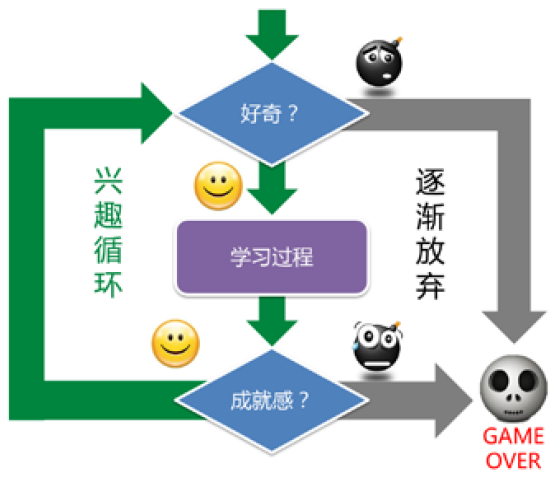
\includegraphics[scale=0.5]{bcing.png}
\caption{图1 正向兴趣循环是学习的关键}
\label{bcing}
\end{figure}

我认为这张图道出了问题的关键——学习过程中的“正向”兴趣循环是否成功地建立。

强烈的兴趣与不断获得的成就感是整个学习过程的“引擎”,它为学生完成整个学习任务提供源源不断的强大动力。有无数的事实支持这个观点。

传统的教学观点认为,本科的主要教育目标之一是为学生在本专业领域未来的发展“打下扎实的理论与实践基础”,所以从一开始就要“严格要求”,“科学训练”。

这个观点不能说错,但我认为,我们的计算机教育,尤其是针对初学者的教育,首要的任务是引发兴趣。没有兴趣,一切免谈。

我所了解的事实是:计算机专业的学生有不少视编程为畏途。其原因在于我们的现有计算机教学方式从一开始就给了这些学生“痛苦”的编程体验,不幸的是,这种体验在后期枯燥的专业课学习中不断得到强化,学生最终对编程敬而远之或畏之如虎。

事实上,教育学研究早己指出,成功的高效的教学应该是这样的:循序渐进,由浅入深,步步为营,兴趣导向。

教师的职责,不是将知识“灌入”学生的大脑,首要的任务是引发学生的兴趣,鼓励他们去探索未知的领域,主动地学习和吸收知识,培养技能,积累经验。在这个学习过程中,教师要成为一名优秀的导航员,给学生绘出航线,鼓励他们出海远航,解决他们在航行中所遇到的困难,并帮助学生建立学习的“正向”兴趣循环。

对编程的“第一印象”很重要啊!由此,引发了一个很有趣的问题——应该选择哪一门语言作为学生的第一门编程语言?

\section{你学的第一门编程语言是什么?}


在国内的大学中,当前大多数选用C作为学生的第一门编程语言。这其实并没有太大的问题,C的重要性无须我多说。其实问题的关键不在于选择C教学,而在于以哪种方式去教。

很不幸,国内许多C语言的教材都将主要的精力放在对C语法细节的介绍上,课程考核方式又很古板——很多院校采用闭卷考试,出一堆的选择题和填空题。典型的题目是将一段代码砍掉一两句,让学生“填空”。有哪位高手是通过做这些“填空题”学会编程的?上机也流于形式,让学生反复折腾几个“黑底白字”的“玩具般的”小程序,学了一个学期,学生连一个有点用的程序都写不出来……

这种僵化的教学方式,足以毁掉多数学生对编程的兴趣。

 我个人认为,C不应该成为针对大多数学生所讲授的第一门编程语言,我们的教学体系,应该给学生提供更多的选择。

针对初学者所讲授的第一门编程语言,应该具有以下的特点:

\begin{compactenum}
\item 必须是“有趣”的,能诱导人去“动手”和“思考”。
\item 需要对初学者屏蔽不必要的底层技术细节,以免分散他们的注意力。
\item 这种语言必须足够简单,但同时又具备足够的能力编写出实用的程序,从而让学生能比较容易地获得成就感,感悟到软件开发的魅力。
\item 这种语言必须能充分地体现现代软件开发的基本思想和技术成果,为学生进一步深入学习打下基础
\item 花在这门编程语言上的时间和精力是有回报的,掌握了它,就掌握了一个强大的工具,可以在今后的学习中使用这个工具进行实践和创造。
\end{compactenum}

另外,这门编程语言的学习,应该有助于初学者正确理解与体会到以下的编程思想:

\begin{compactenum}
\item 分而治之:将大问题切分为小问题。
\item 组件化与模块化:以搭积木的方式“构建”出软件系统。
\item 算法思想:针对实际问题建立数学模型,设计计算机算法,最终编程解决问题。
\end{compactenum}

同时,这门编程语言的学习,应能有效地培养出以下的编程基本功:

\begin{compactenum}
\item 调试代码的能力。
\item 撰写可读性强、扩充性好、易于复用的优质代码的能力,培养良好的编程习惯。
\item 查找技术资源与阅读技术文档的能力。
\end{compactenum}

也许一门编程语言的学习无法达到上述的所有要求,但组合几种不同的编程语言就差不多了。下面,我介绍几种适合于初学者入门的编程语言。

\section{适合于入门的脚本编程语言}

为了教初学者学会编程,蔡学镛先生的《编程ING》选择了REBOL编程语言,这个语言确实比较简单,而且蔡先生的书图文并貌,用它来训练编程的基本技能很合适,但REBOL这门语言似乎过于小众化了一些,而且书中缺乏有力的能引发初学者兴趣的应用实例。

依据我的经验,如果初学者能动手写出几个有用的实例,他喜欢上编程的可能性会大大增加。

以下是我粗略归纳的很容易引发学生成就感的几个技术领域:

\begin{compactenum}
\item 图形图像与动画、多媒体
\item 游戏
\item 网络应用
\item 拥有可视化界面的桌面应用程序
\item 能跑在手机上的应用程序
\end{compactenum}


就我个人看法,第一门语言比较适合采用脚本式的编程语言。


\subsection{Python:认识编程是怎么回事,训练基本编程技能}

国外有许多人非常推崇Python(http://www.python.org),认为它是最适合初学者学习的一门编程语言。

Python是一种动态编程语言,语法简洁易学,本身是开源的,Python程序可以运行于几乎所有主流的操作系统之上。

对于初学者而言,使用Python可以学习基本的编程知识(比如学会编写分支、循环语句),体会动态编程语言的特点,并理解类和对象等面向对象编程的基本知识。

但针对国内的实际情况,使用Python存在着一些问题:

\begin{compactenum}
\item 官方提供了一个交互式的开发环境IDLE,易于使用,但要开发拥有可视化界面的程序比较麻烦,其他厂商的开发环境也不太成熟稳定。

\item 缺少合适的中文教材,与其他语言相比,在国内应用也并不算广。  个人观点:使用Python对初学者进行基本编程技能的训练还是比较合适的,但在使用它入门之后,还必须学习其他的编程语言。
\end{compactenum}


\subsection{MATLAB和Scilab:训练算法的设计与编程实现能力}


学习、应用和设计各种算法,培养为各种问题建立数学模型的能力,这对于软件开发而言非常重要,我国己在高中数学教学中引入了算法,并将其纳入了高考的考试内容,这是件好事。

当前高中新课标数学课本中,使用的是由法国国家信息自动化研究院(INRIA)开发的Scilab(http://www.scilab.org/),这个软件与大学里流行的MATLAB高度类似,是学习算法的好工具。

比较遗憾的是,Scilab也缺少足够的中文资料,并且由于高考数学仅考察简单的算法流程图,占分很少,因此大多数的高中都不会对这块投入太大力气,学生的算法思想和数学建模能力无法得到比较充分的训练,这个任务只能留到大学来完成了。

使用Scilab或MATLAB作为第一门编程语言是完全可以的,与Python类似,Scilab或MATLAB编程采用交互式的运行方式(图2),编程语法也很简易,通过它同样能培养出基本的编程技能,特别是它们强大的数学图形功能,对学生吸引力很强,Scilab或MATLAB编程对他们数学能力与算法设计应用能力的训练无以伦比,这种能力会为学生未来在学术研究领域的发展提供强劲动力。

\begin{figure}[!h]
\centering
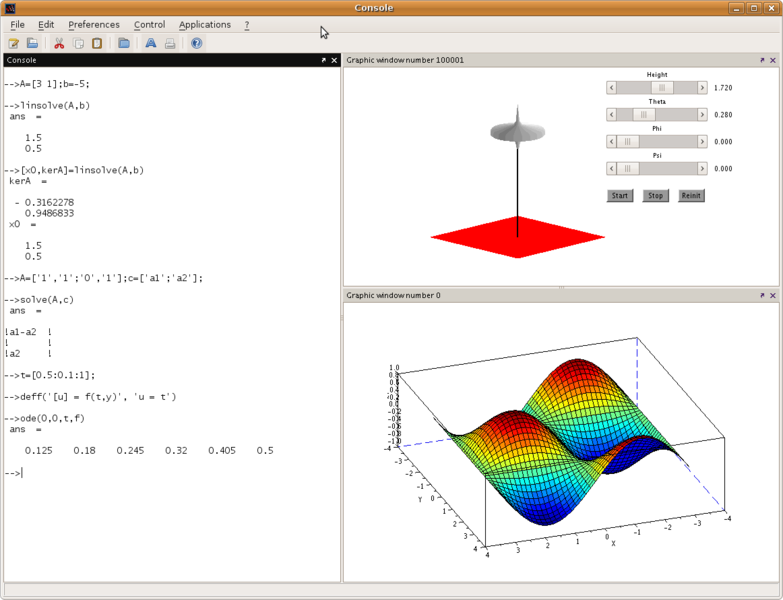
\includegraphics[scale=0.5]{scilab.png}
\caption{图2  Scilab交互式编程环境}
\label{scilab}
\end{figure}


\subsection{Office+VBA:用VBA代码控制Office,让各种工作自动化}

几乎所有大学都开设有《计算机基础》这门课程,其中大多都会讲授微软Office软件包的使用。但当前这门课程教学方式是存在问题的,比如我看到过一些考试试题,考核学生是否记住了Word的某些操作快捷键,这完全是本末倒置!其实,将本课程教学内容略作改革,完全可以用于培养学生的编程技能,其中的关键在于加强或新增以下几个内容:

\begin{compactenum}
\item 使用Excel进行数据分析,讲授Excel中功能强大的各种函数用法及数据的可视化呈现,这不仅实用,而且能有效地培养学生处理与理解数据的能力,而程序本质上不就是完成信息加工处理的工作吗?
\item 使用Access存储与检索数据,这能让学生掌握数据库使用的基础知识,形成对数据库技术的感性认识。
\item Visual BasicFor Application(VBA)编程:VBA是一种脚本式的编程语言,在Office软件包中具有“控制一切”的能力,使用它进行编程的最大好处时能让学生体会到——原来很多操作均可以一键“自动化”,并且在实现这种“自动化”的过程中拥有成就感。
\end{compactenum}

\subsection{Processing编程语言:体会图形与动画的魅力}

国内可能有很多人不知道Processing这个编程语言(http://www.processing.org/),其实它己有10多年的历史,由美国CaseyReas教授与 Ben Fry所设计,可用于构造丰富多彩的交互式应用软件。

与其它编程语言相比,Processing最强悍之处在于它的图形图像及动画编程功能。而在整个计算机技术领域中,这一块无疑是最吸引人的技术领域之一。

虽说磨刀不误砍柴功,但有不少编程语言在能够真正“砍柴(即动手开发真正有用的程序)”之前,需要太长的时间“磨刀(学习语法,掌握开发工具、阅读API文档等等)”,而Processing就不存在这个问题,它的编程语法与Java一致,但比Java简洁得多,另外,与复杂的IDE如Eclipse、Visual Studio之类相比,Processing的编程环境非常简单,这有助于学习者将主要精力用于创作上,并鼓励他们大胆地进行开发实践。

\begin{figure}[!h]
\centering
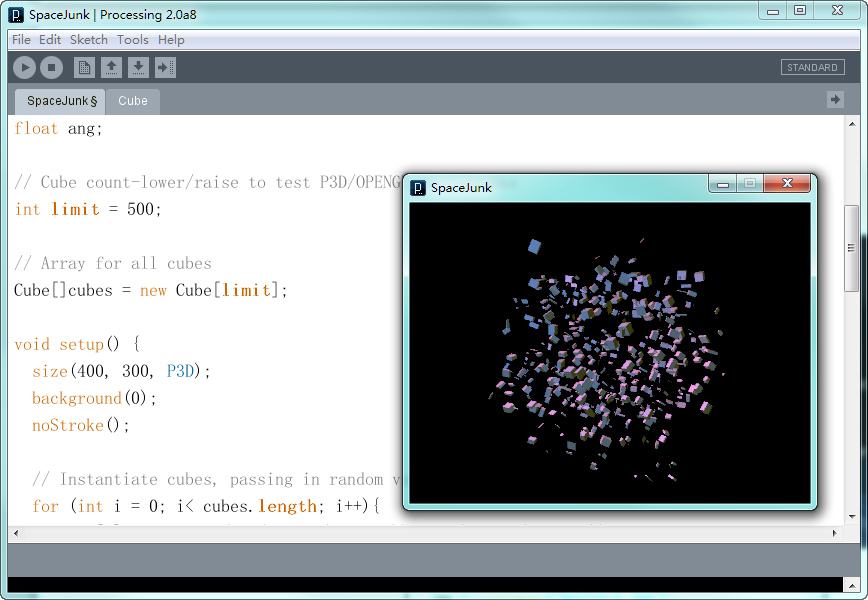
\includegraphics[scale=0.5]{processing.png}
\caption{图3 Processing编程环境}
\label{processing}
\end{figure}

Processing提供了一批直观、简洁而功能强大的图形图像函数,学习者仅需花少量时间学习就能立即投入到创作之中,而它所提供的大量可运行实例,能有效地激发学习者的想象力。

Processing具有很强的可扩展性(现在已经有一百多个库可用了),特别地,Processing内置了对于Android的支持,Processing程序能够跑在Android手机上,这大大地增加了它的吸引力。

也许不少国内高校目前还无法开设Processing课程,但事实上大学生们是完全可以自学的,Processing网站上有足够的学习资源和示例,唯一比较遗憾的是这些资源都是英文的。


\subsection{Small Basic:适合“零编程基础”人的编程语言}

在中国,有不少人是通过Basic语言迈入编程的大门的,特别是微软在上个世纪所推出的Visual Basic,更被视为Windows桌面编程最佳入门语言,只可惜这个优势在其后继版本Visual Basic.NET中己经不复存在,从功能上说,现在的Visual Basic.NET与C\#基本一致,付出的代价是Visual Basic.NET语言本身的复杂程度也变得与C\#是同一级别的了,而后者的使用者要比前者多得多,与其学Visual Basic.NET,不如直接学C\#。

这里,我想介绍的是微软所推出的另一种Basic编程语言——SmallBasic(http://www.smallbasic.com/)。

微软公司在其软件用户友好性方面一直做得非常出色,Small Basic沿袭了这个特色,其开发环境的易用性超过前面介绍的所有编程语言,并提供智能的编程帮助(图4)。

\begin{figure}[!h]
\centering
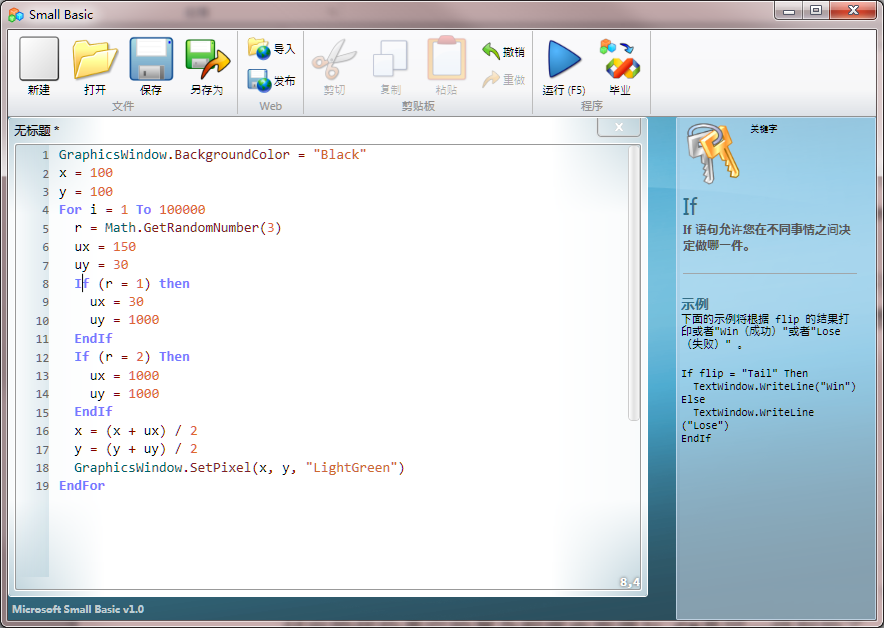
\includegraphics[scale=0.5]{small_basic.png}
\caption{图 4 Small Basic的智能编程环境}
\label{small_basic}
\end{figure}

Small Basic提供了两个强大的“窗口”对象——TextWindow(用于输出文本)和GraphicsWindow(用于绘图),特别有趣的,它从历史悠久的Logo语言中得到借鉴,提供了一个小乌龟(Turtle)对象,通过简单的指令就可以命令这只小乌龟(Turtle)在屏幕上“爬”出各种图案来,确实有趣好玩。

我个人看法,Small Basic是一个非常好的针对“零基础”人的入门编程语言,特别适合于年纪较小的学习者(比如初高中学生),也可供非计算机专业(比如文科专业)的大学生编程快速入门。


\subsection{HTML 5 + JavaScript:互联网时代的主流编程语言}

各种脚本编程语言中,我想介绍的最后一种是JavaScript。

JavaScript早就是Web客户端事实上的主流编程语言,它的运行环境是浏览器,当前所有的计算机和绝大部份智能手机都至少安装有一种浏览器,JavaScript程序“到处都可以运行”。

JavaScript程序的编写极为简单,就算使用Windows记事本,写上几段也不算太麻烦。

JavaScript早期存在的问题主要是各浏览器厂商自行其是,标准不统一,而且缺少必要的调试工具,但这些问题现在己大大缓解。以开发工具来说,主流的IDE纷纷加入对JavaScript程序开发与调试的支持,比如Visual Studio 2010/2012就做得很出色,另外,随着我们进入移动互联网的时代,HTML 5是唯一能被各厂商接受的标准,与此对应,JavaScript也正在走向标准化。

与Python等语言类似,JavaScript也可归入动态脚本语言的范畴,语法简单,同样支持面向对象的编程方式,但JavaScript的使用远比Python等语言广,诸如jQuery之类的各种JavaScript库如雨后春笋般地出现,其功能无所不包,甚至在服务端JavaScript也大展身手,比如一个事件驱动的服务端JavaScript运行环境——Node.js(http://nodejs.org/)就相当引人注目。

JavaScript在HTML 5规范中拥有核心的地位,可以用JavaScript完成很多的工作:

\begin{compactitem}
\item 基于canvas可编程绘制二维的图形,使用SVG通过DOM可构造交互式的应用
\item  HTML 5的audio和video元素可以播放音频和视频,所以可以用JavaScript开发多媒体应用
\item  Geolocation、Communication和WebSocket  API支持编写地理感知的互联网应用程序
\item  ……
\end{compactitem}

为了抢战先机,各大浏览器厂商都在不断地完善自己的产品,争取能支持更多的HTML 5特性,而且智能手机的两大主流操作系统iOS和Android都可以运行使用JavaScript编写的Web应用。微软也在紧跟这个潮流,在其最新的Windows 8中,可以使用JavaScript编写Metro风格的Windows 8 应用。

由此看来,JavaScript可谓是风光无限。

我强力推荐在高校中推广JavaScript课程,其实国内高校在这方面也已经有一定基础了,比如许多高校都开设有《网页设计基础》这门课程,只需更新一下课程的教学内容,加入HTML 5和JavaScript的内容,并改革教学方式(比如千万不要再采用闭卷考试的方式要学生去背各种HTML标记的含义……),就能让学生跟上时代的步伐,而且我相信JavaScript一定会比C更能吸引学生,激发他们对软件开发的兴趣。

\section{以编译型的语言作为入门级编程语言}

虽然我更趋向于使用脚本语言完成初学者的编程启蒙任务,但我们同样可以使用编译型的编程语言完成这一任务。

C就不用我多说了,相信有很多牛人是从C出来的。

另两门非常重要的编译型语言是Java和C\#,我的看法是即使不把它们当成计算机专业的第一门编程语言,至少也应该在计算机专业一、二年级安排这两个编程语言的选修课程。

下面先说说Java。



\subsection{Java:“人多势众”的主流面向对象编程语言}

据说全世界的软件开发人员中,Java程序员的总人数名列前茅。人多说明市场需求量大,Java技术应用广。

采用Java作为第一门编程语言,比较适合于计算机专业的学生,能让他们一开始就能受到面向对象编程风格与思想的熏陶,之后他们可以再倒过来去学C。而不是象现在这样,先学C再学Java,谈到C再顺便说说C++,现在许多院校开设有C++课程,其实这些年来C++应用的领域被不断地压缩,而且C++语法过于复杂,开发效率低,除了部分有需求有兴趣的学生,不适合多数学生学习。

Java入门主要分为两个阶段:一是Java语法与OOP思想的领悟,二是JDK中各个Java类及相关技术(比如多线程、序列化等)的学习。

Java是Android的主要开发语言,因此学生在入门之后,可以进一步地开发基于Android的手机应用,引导学生进入移动互联的时代,具有很强的实用性,这点往往能触发学生学习Java的强劲动力。

Java天生与“开源”两字联系在一起,掌握Java之后,学生可以迈入开源的世界,探索各种丰富的开源应用和技术的奇思妙想,这对于开拓学生的视野非常有好处,并且能直接地帮助其就业。

其实很多院校都开设了Java课程,我的建议不过就是将其提到大学一年级就讲授,并立即跟上J2EE和Android的后继课程。

\subsection{C\#:面向对象编程语言的集大成者}

作为面向对象编程语言家族的后来者,C\#有足够的机缘从前辈中汲取经验,这使得C\#成为一个面向对象编程语言的集大成者。

与Java类似,C\#比较适合作为计算机专业的入门级编程语言。C\#开发通常使用微软自己研发的Visual Studio,与其他IDE相比,我认为Visual Studio是非常优秀的集成开发环境,即使是免费的版本,也拥有高度的智能性和良好的使用体验。

笔者曾经做过试验,直接带领计算机专业一年级学生在没有学C的前提下学习C\#,也开设过全校的通识选修课,针对非计算机专业的学生讲授C\#编程语言与.NET编程技术,都得到了良好的反馈。

以下是我总结出来的C\#编程中几个很能引发学生兴趣的内容:

\begin{compactenum}
\item Windows Forms:可让学生迅速地开发出可视化的桌面应用程序,极具成就感。
\item GDI+:通过简单的循环、递归的编程技巧,能够绘出漂亮的图案,并且可以移植到Web上,很吸引学生。
\item ADO.NET:掌握它学生就可以开发简单的数据库应用程序,真正地写出一些有用的程序。
\item Socket编程:让学生轻易地实现两台计算机互相交换信息,这个过程充满探索的乐趣。
\end{compactenum}

以上几板斧下来,实践证明,能成功地引发很多学生对编程的兴趣,甚至“引诱”了不少学生决定跨专业报考计算机专业的研究生。

与Java相比,C\#的问题是与微软公司绑得太紧,容易把学生局限于微软所构建的生态系统之中,影响其视野的开阔性。

就我个人观点,计算机专业的学生应该在大一,最晚推迟到大二,就掌握一门主流的通用型编程语言和开发工具(Java和C\#是我当前推荐的两种编程语言),并且在今后的专业学习中,使用它们把在后继计算机专业课中学到的理论知识应用于实践。这样一来,编程语言的学习就给计算机专业理论课的学习以强劲的推动,而学生的开发能力也将随着开发实践的深入而不断增强,为其日后迈入业界或进入学术领域铺路。

\section{结束语:与时俱进的计算机教学}

计算机是进步最快的技术领域之一,这就要求我们的计算机教学应该与时俱进并不断地调整。笔者从《计算机学会通讯》2012年第6期的一篇文章了解到,美国加州大学伯克利分校己经开设了这样的课程:教学生使用Ruby On Rails之类的工具进行敏捷开发并在Amazon web Services上部署。

“云计算”来了!

 “云计算”时代的来临,会对计算机教学的方式产生巨大的影响,笔者设想了一下,如果由教育部牵头,由国家投资支持组建一个“教育与科研云”,打造一个国家级的教育公共平台,不走商业化的路,坚持让所有的在校学生和教师都能免费使用,努力推动各种的教学资源上移到云端,让更多的课程能用上云平台所提供的丰富资源与强大计算能力,这将是一项利国利民的教育基础设施建设,从长远来说,对人的教育投资,是收益最大的投资。已经成为世界第二大经济体的中国,难道还拿不出这笔钱和资源进行这个旨在为整个民族赢得未来的长线投资?

21世纪是人类信息技术突飞猛进并全面渗透到人类社会各领域的时代,在这样一个日益信息化的时代里,

\bibliographystyle{plainnat}
\bibliography{gk}
\clearpage







